In this chapter we consider model-free learning algorithms. The main
idea of model-free algorithms is to avoid learning the MDP model
directly. The model based methodology was the following. During the
learning we estimate model of the MDP, and later,  we derive the
optimal policy of the estimated model. The main point was that an
optimal policy of a near-accurate MDP is an near-optimal policy in
the true MDP.

The model-free methodology is going to be different. We will never
learn an estimated model, but rather we will directly learn the
value function of the MDP. The value function can be either the
$\QValue$-function (as is the case in Q-learning and SARSA) or the
$\Value$-function (as is the case in Temporal Difference (TD) algorithms
and the Monte-Carlo approach).

We will first look at the case of deterministic MDPs, and develop a Q-learning algorithm that learns the $\QValue$-function directly from interaction with the MDP. We will then extend our approach to general MDPs, where our handling of stochasticity will be based on the \textit{stochastic approximation} technique. We will first look at learning $\Value^{\policy}$ for a fixed policy, using either temporal difference on Monte-Carlo methods, and then look at learning the optimal $\QValue$-function, using the Q-learning and SARSA methods. At the end of the chapter we have a few miscellaneous topics, including,
evaluating one policy while following a different policy (using
importance sampling) and the actor-critic methodology.

\section{Model Free Learning -- the Situated Agent Setting}

The learning setting we consider involves an agent that sequentially \textit{interacts} with an MDP, where by interaction we mean that at time $\ttime$ the agent can observe the current state $\state_{\ttime}$, the current action $\action_{\ttime}$, the current reward $\reward_{\ttime} = \reward(\state_{\ttime},\action_{\ttime})$, and the resulting next state $\state_{\ttime+1} \sim \transitionkernel(\cdot | \state_{\ttime},\action_{\ttime})$. Throughout the interaction, the agent collects \textit{transition tuples}, $\left(\state_{\ttime}, \action_{\ttime}, \reward_{\ttime}, \state_{\ttime+1} \right)$, which will effectively be the \textit{data} used for learning the value MDP's value function. That is, all our learning algorithms will take as input transition tuples, and output estimates of value functions. For some algorithms, the time index of tuples in the data is not important, and we shall sometimes denote the tuples as $\left(\state, \action, \reward, \state' \right)$, understanding that both notations above are equivalent.

As with any learning method, the data we learn from has substantial influence on what we can ultimately learn. In our setting, the agent can \textit{control} the data distribution, through its choice of actions. For example, if the agent chooses actions according to a Markov policy $\policy$, we should expect to obtain tuples that roughly follow the stationary distribution of the Markov chain corresponding to $\policy$. If $\pi$ is very different from the optimal policy, for example, this data may not be very useful for estimating $\Value^*$. Therefore, different from the supervised machine learning methodology, in reinforcement learning the agent must consider both how to learn from data, but also how to \textit{collect} it. As we shall see, the agent will need to \textit{explore} the MDP's state space in its data collection, to guarantee that the optimal value function can be learned. In this chapter we shall devise several heuristics for effective exploration. In proceeding chapters we will dive deeper into how to provably explore effectively.


\section{ $\QValue$-learning: Deterministic Decision Process}\label{sec:q_learning_DDP}

The celebrated $\QValue$-learning algorithm is among the most popular and fundamental model-free RL methods.
To demonstrate some key ideas of $\QValue$-learning, we start with a
simplified learning algorithm that is suitable for a {\em
Deterministic Decision Process (DDP)} model, namely:
\begin{align*}
& \state_{\ttime+1}=f(\state_\ttime,\action_\ttime) \\
& \reward_\ttime=\reward(\state_\ttime,\action_\ttime)
\end{align*}
We consider the discounted return criterion:
\begin{align*}
\Value^{\policy}(\state) &=\sum_{\ttime=0}^\infty \discount^\ttime
\reward(\state_\ttime,\action_\ttime)\,,
\quad \text{given } \state_0=\state, \action_\ttime=\policy(\state_\ttime)\\
\Value^*(\state) &= \max_\policy \Value^\policy(\state),
\end{align*}
where $\Value^*$ is the value function of the optimal policy.

Recall our definition of the $Q$-function (or {\em state-action
value function}), specialized to the present deterministic setting:
$$
\QValue^*(\state,\action)=\reward(\state,\action)+\discount
\Value^*(f(\state,\action))
$$
The optimality equation is then
$$
\Value^*(\state) = \max_\action \QValue^*(\state,\action),
$$
or, in terms of $\QValue^*$:
$$
\QValue^*(\state,\action)=\reward(\state,\action)+\discount
\max_{\action'}\QValue^*(f(\state,\action),\action').
$$

The $\QValue$-learning algorithm runs as follows:
\begin{itemize}
\item {\em Initialize:} Set $\widehat{\QValue}(\state,\action)=0$, for all $\state$, $\action$.
\item At time $\ttime=0,1,\dots$:

-- Select action $\action_\ttime$

-- Observe $(\state_\ttime$, $\action_\ttime$, $\reward_\ttime$,
$\state_{\ttime+1}),$
% where $\reward_\ttime$ is the observed reward
% when executing action $\action_\ttime$ in state $\state_\ttime$ and
% $\state_\ttime'$ is the next state, i.e.,
where here $\state_{\ttime+1}=f(\state_\ttime,\action_\ttime)$.
% $s\leftarrow \state_n$, $a \leftarrow \action_n$, $r\leftarrow \reward_n$, $s'\leftarrow \state_{n+1}$.

-- Update:\ \ \
$\widehat{\QValue}_{\ttime+1}(\state_\ttime,\action_\ttime) :=
\reward_\ttime+\discount \max_{\action'}
\widehat{\QValue}_\ttime(\state_{\ttime+1},\action')$.
\end{itemize}

The update in $\QValue$-learning is an example of a technique that is often termed ``bootstrapping''\footnote{Related to the saying ``to pull oneself up by one's bootstraps''.}, where we use our current, and possibly inaccurate value estimate $\widehat{\QValue}_\ttime$, to improve the accuracy of the same value function. The intuition for why this makes sense comes from the discount factor: since in the update $\reward_\ttime+\discount \max_{\action'}
\widehat{\QValue}_\ttime(\state_{\ttime+1},\action')$ the first term is accurate (the reward is not estimated), and the second term is multiplied by the discount factor, we expect that if $\discount<1$ our updated value would suffer less from the inaccuracy. 

The $\QValue$-learning algorithm is an off-policy algorithm, namely, it does specify how to choose the actions
$\action_\ttime$, and this can be done using various exploration methods.
To guarantee convergence of $\QValue$-learning, we will need to have some assumption about the
sequence of actions selected, as is the case in the theorem below. We shall later discuss exploration methods that satisfy this assumption.
% The following result is from [Mitchell, Theorem 3.1].

\begin{theorem}[Convergence of $\QValue$-learning for DDP]\ \\
Assume a DDP model.
%Let $\widehat{\QValue}_\ttime(\state,\action)$ denote the estimated $Q$-function before the $\ttime$-th update.
If each state-action pair is visited {\em infinitely-often}, then
$\lim_{\ttime\to\infty}\widehat{\QValue}_\ttime(\state,\action)=\QValue^*(\state,\action)$,
for all $(\state,\action)$.
\end{theorem}

\begin{proof}
The proof would be done by considering the maximum difference between $\widehat{\QValue}_\ttime$ and $\QValue^*$.
Let
\[
\Delta_\ttime \dfn \|\widehat{\QValue}_\ttime-\QValue^*\|_\infty =
\max_{\state,\action}
|\widehat{\QValue}_\ttime(\state,\action)-\QValue^*(\state,\action) | \,.
\]
The first step is to show that after an update at time $\ttime$ the difference at the updated state-action $(\state_\ttime,\action_\ttime)$ between $\widehat{\QValue}_\ttime$ and $\QValue^*$ can be bounded by $\discount \Delta_\ttime$. This does not imply that $\Delta_{\ttime}$ would shrink, since it is the maximum over all state-action pair. Later we show that eventually, after we update all state-action pairs at least once, then we are guaranteed to have the difference shrink by a factor of at least $\discount$. 

First, at every stage $\ttime$:
\begin{align*}
| \widehat{\QValue}_{\ttime+1}(\state_\ttime,\action_\ttime)-
\QValue^*(\state_\ttime,\action_\ttime)| &=
\big|(\reward_\ttime+\discount\max_{\action'}
\widehat{\QValue}_\ttime(\state_{\ttime}',\action'))
- (\reward_\ttime+\discount\max_{\action''} \QValue^*(\state_{\ttime}',\action'') ) \big| \\
&= \discount |\max_{\action'} \widehat{\QValue}_\ttime(\state_{\ttime}',\action') -\max_{\action''} \QValue^*(\state_{\ttime}',\action'') | \\
& \le \discount \max_{\action'}
|\widehat{\QValue}_\ttime(\state_{\ttime}',\action') -
\QValue^*(\state_{\ttime}',\action') | \\
&\le\; \discount \Delta_\ttime
\,.
\end{align*}
where the first inequality uses the fact that $|\max_{x_1} f_1(x_1)-\max_{x_2}f(x_2)|\leq \max_x|f_1(x)-f_2(x)|$, and the second inequality follows from the bound on $\|\widehat{\QValue}_\ttime-\QValue^*\|_\infty =\Delta_t $.
This implies that the difference at $(\state_\ttime,\action_\ttime)$ the errors is bounded by $\discount\Delta_\ttime$, but this does not imply that $\Delta_{\ttime+1}\leq \discount\Delta_{\ttime}$, since it is the maximum over all state-action pairs.

Next, we show that eventually $\Delta_{\ttime+\tau}$ would be at most $ \discount\Delta_{\ttime}$.
Consider now some interval $[\ttime,\ttime_1]$ over which all state-action pairs $(\state,\action)$ appear at least once. Using the above relation and simple induction, it follows that $\Delta_{\ttime_1} \le \discount \Delta_{\ttime}$.
%
Since each state-action pair is visited infinitely often, there is
an infinite number of such intervals, and since $\discount<1$, it
follows that $\Delta_\ttime \to 0$, as $\ttime$ goes to infinity.
\end{proof}

\begin{remark}
Note that the $\QValue$-learning algorithm does not need to receive a continuous trajectory, but can receive arbitrary quadruples
$(\state_\ttime,\action_\ttime,\reward_\ttime,\state_{\ttime}')$. We do need that for any state-action pair $(\state,\action)$ we have infinitely many times $\ttime$ for which $\state_\ttime=\state$ and $\action_\ttime=\action$.
\end{remark}

\begin{remark}\label{remark:modelfree_Q_learning_step}
We could have also relaxed the update to use a step-size $\alpha\in (0,1)$ as follows: $\widehat{\QValue}_{\ttime+1}(\state_\ttime,\action_\ttime) := (1-\alpha) \widehat{\QValue}_{\ttime}(\state_\ttime,\action_\ttime) + \alpha \left(
\reward_\ttime+\discount \max_{\action'}
\widehat{\QValue}_\ttime(\state_{\ttime+1},\action')\right)$. The proof follows similarly, only with a bound $| \widehat{\QValue}_{\ttime+1}(\state_\ttime,\action_\ttime)-
\QValue^*(\state_\ttime,\action_\ttime)| \leq \left( 1 - \alpha(1 - \discount)\right) \Delta_\ttime$, and it is clear that $\left( 1 - \alpha(1 - \discount)\right)<1$ when $\discount<1$. For the deterministic case, there is no reason to choose $\alpha<1$. However, we shall see that taking smaller update steps will be important in the non-deterministic setting.
\end{remark}

\remove{
\section{Online approximation of mean}

Before we start looking at model-free learning algorithms, we look
at a very simple task, approximating the average of a random
variable using samples. Our main goal would be to do it in an online
way while maintaining minimal information, namely the average.

Assume we have a random variable $Z\in [0,1]$ with $\mu=\E[Z]$. We
observe $m$ samples, $z_1, \ldots , z_m$. In the batch setting we
simply compute the average of the samples,
$\widehat{\mu}_m=(1/m)\sum_{i=1}^m z_i$. We can bound
$|\mu-\widehat{\mu}_m|$ using Chernoff-Hoeffding concentration
bounds (see Lemma~\ref{lemma:chernoff}).

We can actually perform the computation of the average in an online way:
\[
\widehat{\mu}_m=\frac{1}{m}\sum_{i=1}^m
z_i=\frac{m-1}{m}\widehat{\mu}_{m-1}+\frac{1}{m}z_m=\widehat{\mu}_{m-1}+\frac{1}{m}(z_m-\widehat{\mu}_{m-1})
\]

This leads naturally to the {\em exponential averaging} where we have
a sequence of $\alpha_t \in(0,1)$ and
% such that $\sum_t \alpha_t=1$ and we have
\[
\bar{\mu}_m=\bar{\mu}_{m-1}+\alpha_m(z_m-\bar{\mu}_{m-1})=\sum_{i=1}^m
\beta_i z_i
\]
where $\beta_i=\alpha_i\prod_{j=i+1}^{m}(1-\alpha_j)$. Note that $\sum_{i=1}^m \beta_i=1$. The regular averaging is a special case with $\alpha_i=1/i$ and $\beta_1=1/m$.

We would like to show that the approximation $\bar{\mu}$
concentrates around the mean $\mu$. For this we will introduce the
McDiarmid inequality.

The setting of the McDiarmid inequality is the following. There is a
domain $\cX$, which can be for example $\Reals^d$. We have $n$
random variables $X_i \in \cX$. There is a function $f$ which maps
the realization of the $n$ independent (but not necessarily
identical) random variables to a value. Namely, $f:\cX^n \rightarrow
\Reals$.

We define $c_i$, the \emph{sensitivity}  of the function $f$ to the $i$-th
input, to be
$$
c_i =\max_{x\in \cX^n} \max_{a_1,a_0\in X} |f(x_1,
\ldots,x_{i-1},a_0,x_{i+1},\ldots, x_n)-f(x_1,
\ldots,x_{i-1},a_1,x_{i+1},\ldots, x_n)|
$$


The basic idea of McDiarmid's inequality is that with high probability
the observed value of $f$ is close to its expected value. Formally,
\begin{lemma}[McDiarmid's inequality]
\label{lemma:McDiarmid}
\[
\Pr[|f(x)-\E[f(x)|\geq \varepsilon]\leq e^{-2\varepsilon^2/(\sum_i
c_i^2)}
\]
\end{lemma}
%Note that $\sum_i c_i^2$ is an upper bound on $\sum_i VAR(X_i)$.

We can use McDiarmid's inequality to recover the concentration bounds
for a simple average. Define $avg(x_1, \ldots ,
x_n)=(1/n)\sum_{i=1}^n x_i$, where $x_i\in[0,1]$. The sensitivity of
$avg$ to any input $x_i$ is exactly $c_i=1/n$. This implies that
$\sum_i c_i^2=\sum_i 1/n^2=1/n$. Therefore, McDiarmid's inequality
gives us,
\[
\Pr[|avg(x)-\E[avg(x)]|\geq \varepsilon]\leq e^{-2\varepsilon^2n}
\]
Note that the bound is very similar to the Chernoff-Hoeffding bound
(Lemma~\ref{lemma:chernoff}).
%(with a slightly worse constant).

We can now use the McDiarmid's inequality for the weighted average
case. Define $wavg(x_1, \ldots , x_n)=\sum_{i=1}^n \beta_i x_i$,
where $x_i\in[0,1]$ and $\sum_i \beta_i=1$. The sensitivity of
$wavg$ to any input $i$ is exactly $c_i=\beta_i$.
%This implies that $\sum_i c_i^2=\sum_i 1/n^2=1/n$.
Therefore, McDiarmid's inequality gives us,
\[
\Pr[|wavg(x)-\E[wavg(x)]|\geq \varepsilon]\leq
e^{-\varepsilon^2/(\sum_i \beta_i^2)}
\]

For the case of exponential averaging, with a fixed parameter $\alpha$, we have $\beta_i=\alpha(1-\alpha)^{m-i}$. This implies
that
\[
\sum_{i=1}^n \beta_i^2 =
\alpha^2\frac{1-(1-\alpha)^{2m}}{1-(1-\alpha)^2}\approx
\frac{\alpha}{2-\alpha}
\]
Therefore, if we set $\alpha\approx \varepsilon^2/(\log (1/\delta))$
we have an accuracy $\varepsilon$ with confidence $1-\delta$.
}


\section{Monte-Carlo Policy Evaluation}
\label{sec:MC}
We shall now investigate model-free learning in MDPs. We shall start with the simplest setting - policy evaluation, using a simple estimation technique that is often termed Monte-Carlo. 


Monte-Carlo methods learn directly from experience in a model free
way. The idea is very simple. In order to estimate the value of a
state under a given policy, i.e., $\Value^\policy(\state)$, we
consider trajectories of the policy $\policy$ from state $\state$
and average them. The method does not assume any dependency between
the different states, and does not even assume a Markovian
environment, which is both a plus (less assumptions) and a minus
(longer time to learn). (A non-Markovian environment could, for
example, have the reward in a state depend on the number of visits
to the state in the episode.) We will concentrate on the case of an
episodic MDP, namely, generating finite length episodes in each
trajectory. A special case of an episodic MDP is a finite horizon
return, where all the episodes have the same length.

Assume we have a fixed policy $\policy$, which for each state
$\state$ selects action $\action$ with probability
$\policy(\action|\state)$. Using $\policy$ we generate an episode
$(\state_1, \action_1, \reward_1, \ldots ,
\state_k,\action_k,\reward_k)$. The observed return of the episode
is $G=\sum_{i=1}^k \reward_i$. We are interested in the expected
return of an episode conditioned on the initial state, i.e.,
$\Value^\policy(\state)=\E[\sum_{i=1}^k \reward_i |\state_1=\state]$.
Note that $k$ is a random variable, which is the length of the
episode.

Fix a state $\state$, and assume we observed returns $G^\state_1,
\ldots , G^\state_m$, all starting at state $\state$. The
Monte-Carlo estimate for the state $\state$ would be
$\widehat{V}^\policy(\state)=\frac{1}{m}\sum_{i=1}^m G_i^\state$. The main
issue that remains is how do we generate the samples $G^\state_i$
for a state $\state$. Clearly, if we assume we can reset the MDP to
any state, we are done. However, such a \emph{reset assumption} is
not realistic in many applications. For this reason, we do not want
to assume that we can reset the MDP to any state $\state$ and start
an episode from it.

\subsection{Generating the samples}

\paragraph{Initial state only}
We use only the initial state of the episode. Namely, given an
episode $(\state_1, \action_1, \reward_1, \ldots ,
\state_k,\action_k,\reward_k)$ we update only
$\widehat{\Value}^\policy(\state_1)$. This is clearly an unbiased
estimate, but has many drawbacks. First, most likely it is not the
case that every state can be an initial state, what do we do with
such states. Second, it seems very wasteful, updating only a single
state per episode.

\paragraph{First visit}
We update every state that appears in the episode, but update it
only once. Given an episode $(\state_1, \action_1, \reward_1, \ldots
, \state_k,\action_k,\reward_k)$ for each state $\state$ that appears
in the episode, we consider the first appearance of $\state$, say
$\state_j$, and update $\widehat{\Value}^\policy(\state)$ using
$G^\state=\sum_{i=j}^k \reward_i$. Namely, we compute the actual
return from the first visit to state $\state$, and use it to update
our approximation. This is clearly an unbiased estimator of the
return from state $\state$, e.g.,
$\E[G^\state]=\Value^\policy(\state)$.

\paragraph{Every visit}
We do an update at each step of the episode. Namely, given an
episode $(\state_1, \action_1, \reward_1, \ldots ,
\state_k,\action_k,\reward_k)$ for each state $\state_j$ that
appears in the episode, we update each
$\widehat{\Value}^\policy(\state_j)$ using
$G^{\state_j}=\sum_{i=j}^k \reward_i$. We compute the actual
return from every state $\state_j$ until the end and use it to update
our approximation. Note that a state can be updated multiple times
in  a single episode using this approach. We will later show that
this estimator is biased, due to the dependency between different
updates of the same state in the same episode.



\begin{figure}
  % Requires \usepackage{graphicx}
  \begin{centering}
 \includegraphics[width=0.5\textwidth]{figures/2state.png}\\
  \caption{First vs. every visit example}\label{fig:2state}
  \end{centering}
\end{figure}

\paragraph{First versus Every visit:}
%
To better understand the difference between first visit and every
visit we consider the following simple test case. We have a two
state MDP, actually a Markov Chain. In the initial state $\state_1$
we have a reward of $1$ and with probability $1-p$ we stay in that
state and with probability $p$ move to the terminating state
$\state_2$. See Figure~\ref{fig:2state}.

The expected value is $\Value(\state_1)=1/p$, which is the expected
length of an episode. (Note that the return of an episode is its
length, since all the rewards are $1$.) Assume we observe a single
trajectory, $(\state_1,\state_1,\state_1,\state_1,\state_2)$, and
all the rewards are $1$. What would be a reasonable estimate for the
expected return from $\state_1$.

{\tt First visit} takes the naive approach, considers the return from
the first occurrence of $\state_1$, which is $4$, and uses this as
an estimate. {\tt Every visit} considers four runs from state
$\state_1$, we have:
$(\state_1,\state_1,\state_1,\state_1,\state_2)$ with return $4$,
$(\state_1,\state_1,\state_1,\state_2)$ with return $3$,
$(\state_1,\state_1,\state_2)$ with return $2$, and
$(\state_1,\state_2)$ with return $1$. {\tt Every visit} averages
the four and has $G=(4+3+2+1)/4=2.5$. On the face of it, the
estimate of $4$ seems to make more sense. 
\begin{advanced}
We will return to this
example later.

\subsection{First visit}
%Maximum likelihood MDP model}

Consider the First Visit Monte-Carlo updates. Assume that for state
$\state$ we have updates $G_1^\state, \ldots , G^\state_m$. Our
estimate would be
$\widehat{\Value}^\policy(\state)=(1/m)\sum_{i=1}^m G^\state_i$.
Since the different $G^\state_i$ are independent, we can use a
concentration bound, to claim that the error is small. Actually we
will need two different bounds. The first will say that if we run
$n$ episodes, then with high probability we have at least $m$
episodes in which state $\state$ appears. The second will say that if
we have $m$ episodes in which state $\state$ appears, then we will
have a good approximation of the value function at $\state$. For the first part,
we clearly will need to depend on the probability of reaching state
$\state$ in an episode. Call a state $\state$ $\alpha$-good if
the probability that $\policy$ visits $\state$ in an episode is at
least $\alpha$.
%This is summarized in t
The following theorem relates the number of episodes to the accuracy
is estimating the value function.
%summarizes the performance of every visit.

\begin{theorem}
Assume that we execute $n$ episodes using policy $\policy$ and each
episode has length at most $H$. Then, with probability $1-\delta$,
for any $\alpha$-good state $\state$, we have
$|\widehat{\Value}^\policy(\state)-\Value^\policy(\state)|\leq
\lambda$, assuming $n\geq (2m/\alpha)\log(2|\States|/\delta)$ and
$m=(H^2/\lambda^2)\log(2|\States|/\delta)$.
\end{theorem}

\begin{proof}
Let $p(\state)$ be the probability that policy $\policy$ visits
state $\state$ in an episode. Since $\state$ is $\alpha$-good, the
expected number of episodes in which $\state$ appears is
$p(\state)n\geq 2m\log(2|\States|/\delta)$. Using the relative
Chernoff--Hoffding bound (Lemma~\ref{lemma:chernoff}) we have that
the probability that we have at least $m$ samples of state $\state$
is at least $1-\delta/(2|\States|)$.

Given that we have at least $m$ samples from state $\state$ using
the additive Chernoff--Hoffding bound (Lemma~\ref{lemma:chernoff})
we have that with probability at least $1-\delta/(2|\States|)$ that
$|\widehat{\Value}^\policy(\state)-\Value^\policy(\state)|\leq
\lambda$. (Since episodes have return in the range $[0,H]$ we need
to normalize by dividing the rewards by $H$, which creates the $H^2$
term in $m$. A more refine bound can be derived by noticing that the
variance of the return of an episode is bounded by $H$ and not
$H^2$, and using an appropriate concentration bound, say Bernstein
inequality.)

Finally, the theorem follows from a union bound over the bad events.
\end{proof}


Next, we relate the First Visit Monte-Carlo updates to the maximum
likelihood model for the MDP. Going back to the example of
Figure~\ref{fig:2state} and observing the sequence
$(\state_1,\state_1,\state_1,\state_1,\state_2)$. The only unknown
parameter is $p$.

The maximum likelihood approach would select the value of $p$ that
would maximize the probability of observing the sequence
$(\state_1,\state_1,\state_1,\state_1,\state_2)$. The likelihood of
the sequence is, $(1-p)^3p$. We like to solve for
\[
p^* = \arg\max (1-p)^3 p
\]
Taking the derivative we have $(1-p)^3-3(1-p)^2p=0$, which give
$p^*=1/4$.
%
For the maximum likelihood (ML) model $M$ we have $p^*=1/4$ and
therefore $V(\state_1;M)=4$.

In general the Maximum Likelihood model value does not always
coincide with the {\tt First Visit} Monte-Carlo estimate. However we
can make the following interesting connection.

Clearly, when updating state $\state$ using {\tt First Visit}, we
ignore all the episodes that do not include $\state$, and also for
each of the remaining episodes, that do include $\state$, we ignore the
prefix until the first appearance of $\state$. Let us modify the
sample by deleting those parts (episodes in which $\state$ does not
appear, and for each episode that $\state$ appears, start it at the
first appearance of $\state$). Call this the {\em reduced sample}.
%(For more details, see Theorem 5 in \cite{SinghS96})

The maximum likelihood model, given a set of episodes, is simply the
observed model. (We will not show here that the observed model is
indeed the maximum likelihood model, but it is a good exercise for the reader to show it.) 
Namely, for each state-action
pair $(\state,\action)$ let $n(\state,\action)$ be the number of
times it appears, let $n(\state,\action,\state')$ be the number of
times $\state'$ is observed following executing action $\action$ in
state $\state$. The observed transition model is
$\widehat(\state'|\state,\action)=n(\state,\action,\state')/n(\state,\action)$.
Assume that in the $i$-th execution of action $\action$ in state
$\state$ we observe a reward $\reward_i$ then the observed reward is
$\widehat{\reward}(\state,\action)=(1/n(\state,\action))\sum_{i=1}^{n(\state,\action)}
\reward_i$.

\begin{theorem}
\label{thm:MC-ML}
%
Let $M$ be the maximum likelihood MDP for the reduced sample. The
expected value of $\state_0$ in $M$, i.e., $\Value(\state;M)$, is
identical to the {\tt First Visit} estimate of $\state_0$, i.e.,
$\widehat{\Value}^\policy(\state_0)$.
\end{theorem}

\begin{proof}
Assume that we have $N$ episodes in the reduced sample and the sum
of the rewards in the $i$-th episode is $G_i$. The First Visit Monte
Carlo estimate would be
$\widehat{\Value}^\policy(\state_0)=(1/N)\sum_{i=1}^N G_i$.

Consider the maximum likelihood model. Since we have a fixed
deterministic policy, we can ignore actions, and define
$n(\state)=n(\state,\policy(\state))$ and
$\widehat{\reward}(\state,\policy(\state))=\widehat{\reward}(\state)$.
We set the initial state $\state_0$ to be the state we are updating.

We want to compute the expected number of visits $\mu(\state)$ to
each state $\state$ in the ML model $M$. We will show that
$\mu(\state)=n(\state)/N$. This implies that the expected reward for
state $\state_0$ in $M$ would be
\[
\Value^\policy(\state_0;M)=\sum_v \mu(v) \widehat{r}(v)=\sum_v
\frac{n(v)}{N}\frac{1}{n(v)}\sum_{i=1}^{n(v)} \reward_i^v =
\frac{1}{N}\sum_{j=1}^N G_j
\]
where the last equality follows by changing the order of summation
(from states to episodes).

It remains to show that $\mu(\state)=n(\state)/N$. We have the
following identities. For $v\neq \state_0$:
\[
\mu(v)=\sum_u \widehat(v|u)\mu(u)
\]
For the initial state we have
\[
\mu(\state_0)=1+ \sum_u \widehat(\state_0|u)\mu(u)
\]
Note that $n(v)=\sum_u n(u,v)$ for $v\neq \state_0$ and
$n(\state_0)=N+\sum_u n(u,\state_0)$, and recall that
$\widehat(v|u)=n(u,v)/n(u)$. One can verify the identities by
plugging in these values.
\end{proof}

\subsection{Every visit}

The {\tt First Visit} updates are unbiased, since the different
updates are from different episodes. For each episode that update is
an independent unbiased sample of the return.
%
For {\tt Every Visit} the situation is more complicated, since there
are different updates from the same episode, and therefore they are
dependent. The first issue that we have to resolve is how we would like
to average the {\tt Every Visit} updates. Let $G^\state_{i,j}$
be the $j$-th update in the $i$-th episode for state $\state$. Let
$n_i$ be the number of updates in episode $i$ and $N$ the overall
number of episodes.

One way to average the updates is to average for each episode the
updates and average across episodes. Namely,
\[
\frac{1}{N}\sum_{i=1}^N \frac{1}{n_i} \sum_{j=1}^{n_i} G_{i,j}
\]
An alternative approach is to sum the updates and divide by the
number of updates,
\[
\frac{\sum_{i=1}^N\sum_{j=1}^{n_i} G_{i,j}}{\sum_{i=1}^N n_i}
\]
We will use the latter scheme, but it is worthwhile understanding
the difference between the two. Consider for example the case that
we have $10$ episodes, in $9$ we have a single visit to $\state$ and
a return of $1$, and in the $10$-th we have $11$ visits to $\state$
and all the returns are zero. The first averaging would give an
estimate of $9/10$ while the second would give an estimate of
$9/20$.

Consider the case of Figure~\ref{fig:2state}. For a single episode
of length $k$ we have that the sum of the rewards is $k(k+1)/2$,
since there are updates of lengths $k, \ldots , 1$ and recall that
the return equals the length since all rewards are $1$. The number
of updates is $k$, so we have that the estimate of a single episode
is $(k+1)/2$. When we take the expectation we have that
$\E[(k+1)/2]=(1/p+1)/2$ which is different from the expected value of
$1/p$. (Recall that the {\tt Every Visit} updates $k$ times using
values $k,\ldots,1$. In addition, $\E[k]=1/p$ which is also the
expected value.) If we have a single episode then both averaging
schemes are identical.

When we have multiple episodes, we can see the difference between
the two averaging schemes. The first will be biased random variables
of $\E[(k+1)/2]=(1/p+1)/2$, so it will converge to this value rather
than $1/p$. The second scheme, which we will use in {\tt Every
Visit} updates, will have the bias decrease with the number of
episodes. The reason is that we sum separately the returns, and the
number of occurrences. This implies that we have
\[
\E[\Value^{ev}(\state_1)]=\frac{\E[k(k+1)/2]}{\E[k]}=\frac{\E[k^2]+\E[k]}{2\E[k]}=
\frac{2/p^2-1/p+1/p}{2/p}=\frac{1}{p},
\]
since $\E[k^2]=2/p^2-1/p$. This implies that if we average many
episodes we will get an almost unbiased estimate using {\tt Every
Visit}.

We did all this on the example of Figure~\ref{fig:2state}, but this
indeed generalizes. Given an arbitrary episodic MDP, consider the
following mapping. For each episode, mark the places where state
$\state$ appears (the state we want to approximate its value). We
now have a distribution of rewards from going from $\state$ back to
$\state$. Since we are in an episodic MDP, we also have to
terminate, and for this we can add another state, from which we
transition from state $\state$ and have the reward distribution as
the rewards from the last appearance of $\state$ until the end of
the episode.
%We can now reduce collapse other state to a single state.
This implies that we have two states MDP as described in
Figure~\ref{fig:2state-general}.


\begin{figure}
  % Requires \usepackage{graphicx}
  \begin{centering}
  \includegraphics[width=0.5\textwidth]{figures/2state-general.png}\\
  \caption{The situated agent}\label{fig:2state-general}
  \end{centering}
\end{figure}


For this MDP, the value is
$\Value^\pi(\state_1)=\frac{1-p}{p}\reward_1+\reward_2$. The single
episode expected estimate of {\tt Every Visit} is
$\Value^\pi(\state_1)=\frac{1-p}{2p}\reward_1+\reward_2$. The $m$
episodes expected estimate of {\tt Every Visit} is
$V(\state_1)=\frac{m}{m+1}\frac{1-p}{p}\reward_1+\reward_2$. This
implies that if we have a large number of episodes the bias of the
estimate becomes negligible. (For more details, see Theorem 7 in
\cite{SinghS96}.)


\subsubsection*{Every visit and squared loss}

Recall that the squared error is summing over all the observation
the squared error. Assume we have $\state_{i,j}$ as the $j$-th state
in the $i$-th episode, and it has return $G_{i,j}$, i.e., the sum of
the rewards from in episode $i$ from step $j$ until the end of the
episode. Let $\widehat{V}(\state_{i,j})$ be the estimate of {\tt
Every Visit} for state $\state_{i,j}$. (Note that states
$\state_{i,j}$ are not unique, and we can have
$\state=\state_{i_1,j_1}=\state_{i_2,j_2}$.) The square error is
\[
SE=\frac{1}{2}\sum_{i,j} (\widehat{V}(\state_{i,j})-G_{i,j})^2
\]
For a fixed state $\state$ we have
\[
SE(\state)=\frac{1}{2}\sum_{i,j:\state=\state_{i,j}}
(\widehat{V}(\state)-G_{i,j})^2
\]
and the total squared error is $SE=\sum_\state SE(\state)$.

Our goal is to select a value $\widehat{V}^{se}(\state)$ for every
state, which would minimize the SE. The minimization is achieved by
minimizing the square error of each $\state$, and setting the values
\[
\widehat{V}^{se}(\state)=\frac{\sum_{i,j:\state=\state_{i,j}}
G_{i,j}}{|{(i,j):\state=\state_{i,j}}|},
\]
which is exactly the {\tt Every Visit} Monte-carlo estimate for
state $\state$.
\end{advanced}

\subsection{Monte-Carlo control}

We can also use the Monte-Carlo methodology to learn the optimal
policy.
%
The main idea is to learn the $Q^\pi$ function. This is done by
simply updating for every $(\state,\action)$. (The updates can be
either {\tt Every Visit} or {\tt First Visit}.) The problem is that
we need the policy to be ``exploring'', otherwise we will not have
enough information about the actions the policy does not perform.

For the control, we can maintain an estimates of the $Q^\policy$
function, where the current policy is $\policy$. After we have a
good estimate of $Q^\policy$ we can switch to a policy which is
greedy with respect to $Q^\policy$. Namely, each time we reach a
state $\state$, we select a ``near-greedy'' action, for example, use
$\varepsilon$-greedy.

We will show that updating from one $\varepsilon$-greedy policy to
another $\varepsilon$-greedy policy, using policy improvement, does
increase the value of the policy. This will guarantee that we will not cycle, and eventually converge.

Recall that an $\varepsilon$-greedy policy, can be define in the
following way. For every state $\state$ there is an action
$\bar{\action}_\state$, which is the preferred action. The policy
does the following: (1) with probability $1-\varepsilon$ selects action $\bar{\action}_\state$. (2) with probability $\varepsilon$, selects
each action $\action \in \Actions$, with probability
$\varepsilon/|\Actions|$.

Assume we have an $\varepsilon$-greedy policy $\policy_1$. Compute
$Q^{\policy_1}$ and define $\policy_2$ to be $\varepsilon$-greedy
with respect to $Q^{\policy_1}$.

\begin{theorem}
For any $\varepsilon$-greedy policy $\policy_1$, the
$\varepsilon$-greedy improvement policy $\policy_2$ has
$\Value^{\policy_2}\geq \Value^{\policy_1}$.
\end{theorem}

\begin{proof}
Let $\bar{\action}_\state=\arg\max_\action
Q^{\policy_1}(\state,\action)$ be the greedy action w.r.t.
$Q^{\policy_1}$. We now lower bound the value of $Q^{\policy_2}$.
\begin{align*}
E_{\action\sim\policy_2(\cdot|\state)}[Q^{\policy_1}(\state,\action)] &= \sum_{\action \in \Actions} \policy_2(\action|\state) Q^{\policy_1}(\state,\action)\\
&= \frac{\varepsilon}{|\Actions|}\sum_{\action \in \Actions}
Q^{\policy_1}(\state,\action)+(1-\varepsilon)Q^{\policy_1}(\state,\bar{\action}_\state)\\
&\geq \frac{\varepsilon}{|\Actions|}\sum_{\action \in \Actions}
Q^{\policy_1}(\state,\action)+(1-\varepsilon)\sum_{\action \in
\Actions}
\frac{\policy_1(\action|\state)-\varepsilon/|\Actions|}{1-\varepsilon}Q^{\policy_1}(\state,\action)\\
&=\sum_{\action \in \Actions} \policy_1(\action|\state)Q^{\policy_1}(\state,\action)=\Value^{\policy_1}(\state)\\
\end{align*}
The inequality follows, since we are essentially concentrating of
the action that $\policy_1(\cdot|\state)$ selects with probability
$1-\varepsilon$, and clearly $\bar{\action}_\state$, by definition,
guarantees a higher value.

It remains to show, similar to the basic policy improvement, that we have
$$
\Value^{\policy_2} (\state)\geq
\max_\action Q^{\policy_1}(\state,\action)\geq
E_{\action\sim\policy_2(\cdot|\state)}[Q^{\policy_1}(\state,\action)]
\geq \Value^{\policy_1}(\state).
$$

Basically, we need to re-write the Bellman optimality operator to
apply to $\varepsilon$-greedy policies as follows:
\[
(T^*_\varepsilon V)(\state) = \max_\action
[(1-\varepsilon)(\reward(\state,\action)+\discount E_{\state'\sim
p(\cdot |\state,\action)}[V(\state')])+ \varepsilon
(\sum_{\action''}\frac{\varepsilon}{|\Actions|}(\reward(\state,\action'')
+\discount E_{\state''\sim p(\cdot |s,\action'')}[V(\state'')]))]
\]
Clearly $T^*_\varepsilon(V)$ is monotone in $V$, and for
$\Value^{\policy_1}$ we have
$T^*_\varepsilon(\Value^{\policy_1})=T^{\policy_2}(\Value^{\policy_1})$.
Since $ T^{\policy_2}(\Value^{\policy_1}) =
E_{\action\sim\policy_2(\cdot|\state)}[Q^{\policy_1}(\state,\action)]$,
this implies that,
\[
T^{\policy_2}(\Value^{\policy_1})=T^*_\varepsilon(\Value^\policy_1)
\geq T^{\policy_1}(\Value^{\policy_1}) = \Value^{\policy_1}
\]
We can continue to apply $T^{\policy_2}$ and due to the monotonicity
have
\[
(T^{\policy_2})^k (\Value^{\policy_1}) \geq (T^{\policy_2})^{k-1}
(\Value^{\policy_1}) \geq \cdots \geq \Value^{\policy_1}
\]
Since $\lim_{k\rightarrow \infty}(T^{\policy_2})^k
(\Value^{\policy_1}) = \Value^{\policy_2}$ we are done.
\end{proof}

\subsection{Monte-Carlo: pros and cons}

The main benefits of the Monte-Carlo updates are:
\begin{enumerate}
\item Very simple and intuitive
\item Does not assume the environment is Markovian
\item Extends naturally to function approximation (more in future
chapters)
\item Unbiased updates (using {\tt First Visit}).
\end{enumerate}

\noindent
The main drawback of the Monte-Carlo updates are:
\begin{enumerate}
\item Need to wait for the end of episode to update.
\item Suited mainly for episodic environment.
\item Biased updates (using {\tt Every Visit}).
\end{enumerate}

Going back to the Q-learning algorithm in Section \ref{sec:q_learning_DDP}, we see that Monte-Carlo methods do not use the bootstrapping idea, which can mitigate the first two drawbacks, by updating the estimates online, \textit{before} an episode is over. In the following we will develop bootstrapping based methods for model-free learning in MDPs. To facilitate our analysis of these methods, we shall first describe a general framework for online algorithms.

\section{Stochastic Approximation}
\label{sec:stochastic-approximation}

There is a general framework of stochastic approximation algorithms.
We will outline the main definitions and results of that literature.
We later use it to show convergence of online learning algorithms.

The stochastic approximation algorithm takes the following general form:
\begin{equation}\label{eq:stochastic_approx}
X_{\ttime+1} =
X_\ttime+\alpha_\ttime((\safunc(X_\ttime)+\omega_\ttime),
\end{equation}
where $X\in \mathbb{R}^d$ is a vector of parameters that we update, $\safunc$ is a deterministic function, $\alpha_\ttime$ is a step size, and $\omega_\ttime$ is a noise term that is zero-mean and bounded in some sense (that will be defined later).

We will be interested in the long-term behavior of the algorithm in Eq.~\ref{eq:stochastic_approx}, and in particular, whether the iterates $X_\ttime$ can be guaranteed to converge as $\ttime \to \infty$.
Without the noise term, Eq.~\ref{eq:stochastic_approx} describes a simple recurrence relation, with behavior that is determined by the function $\safunc$ and the step size (see Remark~\ref{remark:modelfree_Q_learning_step} for an example). In this case, convergence can be guaranteed if $\safunc$ has certain structure, such as a contraction property. In the following, we separate our presentation to two different structures of $\safunc$. The first is the said contraction, with convergence to a fixed point, while the second relates Eq.~\ref{eq:stochastic_approx} to an ordinary differential equation (ODE), and looks at convergence to stable equilibrium points of the ODE. While the technical details of each approach are different, the main idea is similar: in both cases we will choose step sizes that are large enough such that the \textit{expected} update converges, yet are small enough such that the noise terms do not take the iterates too far away from the expected behavior. The contraction method will be used to analyse the model-free learning algorithms in this section, while the ODE method will be required for the analysis in later chapters, when function approximation is introduced.

\subsection{Convergence via Contraction}
In the flavor of the stochastic approximation we consider here, there is a state space $\States$, and
the iterates update an approximation $X(\state)$ at each iteration, with $\state \in \States$. 
% The updates
% are in the direction of $(HX)(\state)+\omega$ where is a (possibly
% non-linear) operator and $\omega$ is a zero mean bounded noise. 
The iterative algorithm takes the following general form:
\[
X_{\ttime+1}(\state) =
(1-\alpha_\ttime(\state))X_\ttime(\state)+\alpha_\ttime(\state)((HX_\ttime)(\state)+\omega_\ttime(\state)).
\]
%where $H$ is a (possibly non-linear) operator.
This can be seen as a special case of the general stochastic approximation form in Eq.~\ref{eq:stochastic_approx}, where $\safunc(X) = H(X) - X$.

We will mainly look at {\em $(B,\discount)$ well behaved} iterative
algorithms, where $B>0$ and $\discount\in(0,1)$, which have the
following properties:
\begin{enumerate}
\item Step size: For every $(\state,\action)$ we have (1) $\sum_\ttime
\alpha_\ttime(\state,\action)
I(\state_\ttime=\state,\action_\ttime=\action)=\infty $, and (2)
$\sum_\ttime \alpha_\ttime^2(\state,\action)
I(\state_\ttime=\state,\action_\ttime=\action)=O(1)$,
\item Noise: $\E[\omega_\ttime(\state)|h_{\ttime-1}]=0$ and $|\omega_\ttime(\state)|\leq B$, where
$h_{\ttime-1}$ is the history up to time $\ttime$.
\item Pseudo-contraction: There exists $X^*$ such that for any $X$ we have $\|HX-X^*\|_\infty
\leq \discount \|X-X^*\|_\infty$. (This implies that $HX^*=X^*$.
Note that any contraction operator $H$ is also a pseudo contraction, with $X^*$ being the unique fixed point of $H$, cf.~Theorem \ref{chapter-discount:thm:Banach})
\end{enumerate}

The following is the convergence theorem for well behaved iterative
algorithms.

\begin{theorem}[Contracting Stochastic Approximation: convergence]\ \\
\label{thm:stoch-approx}
 Let $X_\ttime$ be a sequence that is generated by a
$(B,\discount)$ well behaved iterative algorithm. Then $X_\ttime$
converges with probability $1$ to $X^*$.
\end{theorem}

We will not give a proof of this important theorem, but we will try
to sketch the main proof methodology.

There are two distinct parts to the iterative algorithms. The part
$(HX_\ttime)$ is contracting, in a deterministic manner. If we had
only this part (say, $\omega_\ttime=0$ always) then the contraction
property of $H$ will give the convergence (as we saw before in Remark \ref{remark:modelfree_Q_learning_step}). The
main challenge is the addition of the stochastic noise $\omega_\ttime$. The
noise is unbiased, so on average the expectation is zero. Also, the
noise is bounded by a constant $B$. This implies that if we average
the noise over a long time interval, then the average should be very
close to zero.

The proof considers the $\|X_\ttime-X^*\|$, and  works in phases. In
phase $i$, at any time $\ttime$ in the phase we have
$\|X_\ttime-X^*\|\leq \lambda_i$.
%In addition $\lambda_{i+1}\leq\lambda_i (1+\discount)/2<\lambda_i$.
%
In each phase we have a deterministic contraction using the operator
$H$. The deterministic contraction implies that
the space contracts by a factor $\discount<1$. Taking into account the step size $\alpha_i$, following Remark \ref{remark:modelfree_Q_learning_step}, let $\tilde{\discount}_i = \left( 1 - \alpha_i(1 - \discount)\right)<1$. We have to take care
of the stochastic noise. We make the phase long enough so that the
average of the noise is less than $\lambda_i (1-\tilde{\discount}_i)/2$ factor. This
implies that the space contracts by
$\lambda_{i+1}\leq\tilde{\discount}_i\lambda_i+(1-\tilde{\discount}_i)\lambda_i/2=\lambda_i(1+\tilde{\discount}_i)/2<\lambda_i $. To complete our proof, we need to show that the decreasing sequence $\lambda_i$ converges to zero.
Without loss of generality, let $\lambda_0=1$. Then we need to evaluate $\lambda_\infty = \prod_{i=0}^{\infty}\left( 1 - \alpha_i\frac{1-\discount}{2}\right)$. We have
\begin{small}
\begin{equation*}
    \exp\left( \log \left( \prod_{i=0}^{\infty}\left( 1 - \alpha_i\frac{1-\discount}{2}\right) \right)\right) = \exp\left(   \sum_{i=0}^{\infty}\log\left( 1 - \alpha_i\frac{1-\discount}{2}\right) \right)\approx \exp\left(   -\frac{1-\discount}{2}\sum_{i=0}^{\infty}\alpha_i \right),
\end{equation*}
\end{small}
which converges to zero for a well-behaved algorithm, due to the first step size rule.
% that as the number of phases increases $\lambda_i<
% ((1+\tilde{\discount}_i)/2)^i$ converges to zero.
%each phase contracts by a constant and eventually we have convergence.

\subsection{Convergence via the ODE method}
Here we will consider the general stochastic approximation form in Eq.~\ref{eq:stochastic_approx}, and we will not limit ourselves to algorithms that update only certain states, but may update the whole vector $X_\ttime$ at every time step. 

The asymptotic behavior of the stochastic approximation algorithm is closely related to the solutions
of a certain ODE (Ordinary Differential Equation), namely
$$
\frac{d}{dt}\theta(t)=\safunc(\theta(t)),
$$
or $\dot{\theta}=\safunc(\theta)$.

Given $\{X_\ttime, \alpha_\ttime\}$, we define a {\em continuous-time} process
$\theta(t)$ as follows.  Let
$$
t_\ttime = \sum_{k=0}^{\ttime-1} \alpha_k\,.
$$
Define
$$
\theta(t_\ttime) = X_\ttime\,,
$$
and use linear interpolation in-between the $t_\ttime$'s.

Thus, the time-axis $t$ is rescaled according to the gains $\{\alpha_\ttime\}$.

\begin{center}
\scalebox{.7}{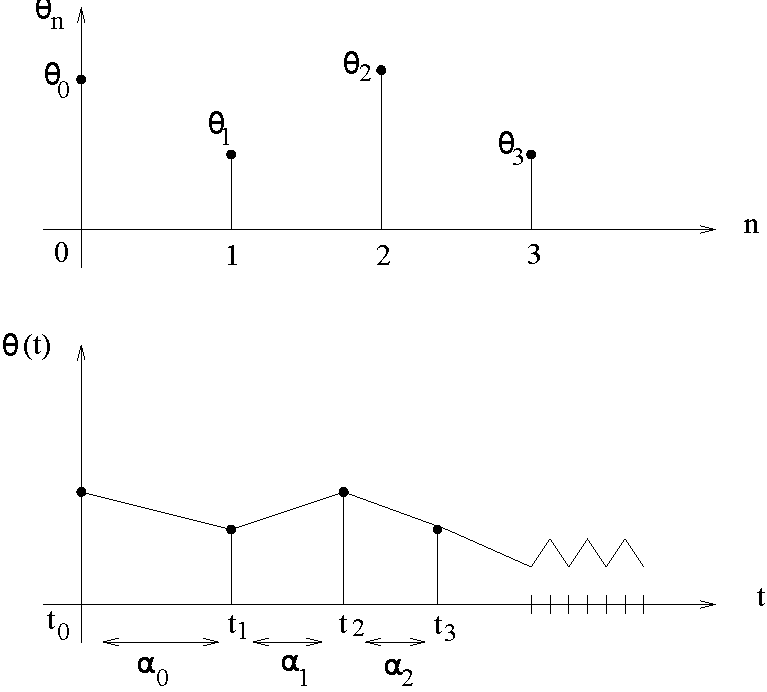
\includegraphics{figures/ch6_fig1a.pdf}}
\end{center}


Note that over a fixed $\Delta t$, the ``total gain'' is approximately
constant:
$$
\sum_{k\in K(t, \Delta t)} \alpha_k \simeq \Delta t\,,
$$
where $K(t,\Delta t) = \{k: t \le t_k < t+ \Delta t\}$.
Plugging in the update of Eq.~\ref{eq:stochastic_approx}, we have
$$
\theta(t+\Delta t) = \theta(t) + \sum_{\ttime\in K(t, \Delta t)} \alpha_\ttime [\safunc(X_\ttime)
+\omega_\ttime] \,.
$$
We now make two observations about the terms in the sum above:
\begin{enumerate}
\item
For large $t$, $\alpha_\ttime$ becomes small and the summation is over many
terms; thus the noise term is approximately ``averaged out'':
$\sum \alpha_\ttime \om_\ttime \to 0$.
\item
For small $\Delta t$, $X_\ttime$ is approximately constant over $K(t, \Delta t):
\safunc(X_\ttime) \simeq \safunc(\theta(t))$.
\end{enumerate}
We thus obtain:
$$
\theta(t+\Delta t) \simeq \theta(t) +\Delta t\cdot \safunc (\theta(t)),
$$
and rearranging gives,
$$
\frac{\theta(t+\Delta t) - \theta(t)}{\Delta t} \simeq  \safunc (\theta(t)).
$$
For $\Delta t \to 0$, this reduces to the ODE:
$$
\dot \theta(t) = \safunc(\theta(t)).
$$

We shall now discuss the convergence of the stochastic approximation iterates.  As $\ttime\to\infty$, we ``expect'' that the estimates
$\{\theta_\ttime\}$ will follow a trajectory of the ODE $\dot\theta=\safunc(\theta)$
(under the above time normalization). Thus, convergence can be expected to \textit{equilibrium points} (also termed \textit{stationary points} or \textit{fixed points}) of the ODE, that is, points $X^*$ that satisfy 
$\safunc(X^*) = 0$. We will also require the equilibrium to be {\em globally asymptotically stable}, as follows.
\begin{definition}
An ODE $\dot \theta(t) = \safunc(\theta(t))$ has a globally asymptotically stable equilibrium point $X^*$, if $\safunc(X^*) = 0$, and
for any $\theta_0$ we have that $\lim_{t \to \infty} \theta(t) = X^*$.
\end{definition}

We will mainly look at {\em $(A,B)$ well behaved} iterative
algorithms, where $B>0$ and $\discount\in(0,1)$, which have the
following properties:
\begin{enumerate}
\item Step size: we have (1) $\sum_\ttime
\alpha_\ttime
=\infty $, and (2)
$\sum_\ttime \alpha_\ttime^2=O(1)$,
\item Noise: $\E[\omega_\ttime(\state)|h_{\ttime-1}]=0$ and $|\omega_\ttime(\state)|\leq A + B\| X_\ttime\|^2$, for some norm $\| \cdot \|$ on $\mathbb{R}^d$, where
$h_{\ttime-1}$ is the history up to time $\ttime$,
\item $\safunc$ is Lipschitz continuous,
\item The ODE $\dot \theta(t) = \safunc(\theta(t))$ has a globally asymptotically stable equilibrium $X^*$,
\item The sequence $X_\ttime$ is bounded with probability 1.
\end{enumerate}
We now give a convergence result.

\begin{theorem}[Stochastic Approximation: ODE convergence]\ \\
\label{thm:stoch-approx-ODE}
 Let $X_\ttime$ be a sequence that is generated by a
$(A,B)$ well behaved iterative algorithm. Then $X_\ttime$
converges with probability $1$ to $X^*$.
\end{theorem}

% \uu{A Remark on Asynchronous Algorithms}:\quad
% When the stepsize is different for each component of $\theta$, the
% approximating ODE is more involved -- the relative rates should enter
% explicitly.
% Still, there exist specifc results that related
% the above ``synchronous'' ODE to the convergence of the
% asynchronous SA algorithm.


\begin{remark}
More generally, even if the ODE is not globally stable, $X_\ttime$ can be shown to converge
to an {\em invariant set} of the ODE (e.g., a limit cycle).
\end{remark}
% \begin{remark}
% Corresponding results exist for the asynchronous versions, under suitable
% assumptions on the relative gains.
% \end{remark}
\begin{remark}
A major assumption in the last result is the boundedness of $(X_\ttime)$.
In general this assumption has to be verified independently. However, there
exist several results that rely on further properties of $\safunc$ to deduce
boundedness, and hence convergence. One technique is to consider the function $\safunc_c(\theta) = \safunc(c \theta) / c$, $c\geq 1$. If $\safunc_c(\theta) \to \safunc_\infty(\theta)$ uniformly, one can consider the ODE with $\safunc_\infty$ replacing $\safunc$~\cite{borkar2009stochastic}. In particular, for a linear $\safunc$, we have that $\safunc_c = \safunc$, and this result shows that boundedness is guaranteed. We make this explicit in the following theorem.
\begin{theorem}[Stochastic Approximation: ODE convergence for linear systems]\ \\
\label{thm:stoch-approx-ODE-linear}
 Let $X_\ttime$ be a sequence that is generated by a
iterative algorithm that satisfies the first $4$ conditions of an $(A,B)$ well behaved algorithm, and $\safunc$ is linear in $\theta$. Then $X_\ttime$
converges with probability $1$ to $X^*$.
\end{theorem}
Another technique to guarantee boundedness
is to use the projected iterates:
$$
X_{\ttime+1} = \text{\it Proj}_\Gamma [X_\ttime+\alpha_\ttime((\safunc(X_\ttime)+\omega_\ttime) ]
$$
where $\text{\it Proj}_\Gamma$ is a projection onto some convex set $\Gamma$.
A simple example is when $\Gamma$ is a box, so that the components of $X$ are simply truncated at their minimal and maximal values. 
If $\Gamma$ is a bounded set then the estimated sequence $\{X_\ttime\}$ is guaranteed
to be bounded. However, in this case the corresponding ODE must account for the projection, and is $\dot \theta(t) = \safunc(\theta(t)) + \zeta$, where $\zeta$ is zero in the interior of $\Gamma$, and on the boundary of $\Gamma$, $\zeta$ is the infinitesimal change to $\theta$ required to keep it in $\Gamma$. In this case, to show convergence using Theorem \ref{thm:stoch-approx-ODE}, we must verify that $X^*$ is still a globally asymptotically stable equilibrium, that is, we must verify that the projection did not add a spurious stable point on the boundary of $\Gamma$. A thorough treatment of this idea is presented in \cite{kushner2003stochastic}.
\end{remark}

\section{Temporal Difference algorithms}
\label{sec:TD}
%In this lecture we will continue looking at model-free learning. In
%the previous lecture we presented: (1) $Q$-learning, which is an
%off-policy learning algorithm that learns the optimal $Q^*$
%function, (2) {\tt SARSA} which is an on-policy variant of
%$Q$-learning where we need to select actions, and (3) Monte-Carlo
%which is a model-free algorithm to learn the value function from
%episodes.

In this section we will look on temporal differences methods, which
work in an online fashion. We will start with $TD(0)$ which uses
only the most recent observations for the updates, and we will
continue with methods that allow for a longer look-ahead, and then
consider $TD(\lambda)$ which averages multiple look-ahead
estimations.

In general, temporal differences (TD) methods, learn directly from
experience, and therefore are model-free methods. Unlike Monte-Carlo
algorithms, they will use incomplete episodes for the updates, and
they are not restricted to episodic MDPs. The TD methods update
their estimates given the current observation and in that direction,
similar in spirit to $Q$-learning and SARSA.

\subsection{TD(0)}

Fix a policy $\policy\in \Pi_{SD}$, stationary and deterministic. The goal
is to learn the value function $\Value^\policy(\state)$ for every
$s\in S$. (The same goal as Monte-Carlo learning.) The TD algorithms
will maintain an estimate of the value function of the policy
$\policy$, i.e., maintain an estimate $\widehat{V}_\ttime(\state)$
for $\Value^\policy(\state)$. The TD algorithms will use their
estimates $\widehat{V}$ for the updates. This implies that unlike
Monte-Carlo, there will be an interaction between the estimates of
different states and at different times.

As a starting point, we can recall the {\em value iteration}
algorithm.
\[
V_{\ttime+1}(\state)=E^\policy[\reward(\state,\policy(\state))+\discount
V_\ttime(\state')]
\]
We have shown that value iteration converges, namely $V_\ttime
\rightarrow_{\ttime\rightarrow\infty} \Value^\policy$.

Assume we sample
$(\state_\ttime,\action_\ttime,\reward_\ttime,\state_{\ttime+1})$.
%Assume that $\policy\in SD$, namely a stationary deterministic policy.
Let $\widehat{V}_\ttime$ our estimation at time $\ttime$,
and we sample
$(\state_\ttime,\action_\ttime,\reward_\ttime,\state_{\ttime+1})$.
Then,
\[
E^\policy[\widehat{V}_\ttime(\state_\ttime)]=
E^\policy[\reward_\ttime+\discount
\widehat{V}_\ttime(\state_{\ttime+1})]=E^\policy[\reward(\state,\action)+\discount
\widehat{V}_\ttime(\state')|\state=\state_\ttime,a=\policy(\state)]
\]
%where $E^\policy [\widehat{V}_\ttime]=V_\ttime$.

The $TD(0)$ will do an update in this direction, namely,
$[\reward_\ttime+\discount \widehat{V}_\ttime(\state_{\ttime+1})]$.

\paragraph{$TD(0)$ Algorithm}

\begin{itemize}
\item \emph{Initialize:} $\widehat{V}(\state)$ arbitrarily.

\item At time $\ttime=0,1,\dots$:


-- Observe: $(\state_\ttime, \action_\ttime, \reward_\ttime,
\state_{\ttime+1})$.

-- Update:
%$(\state_\ttime,\action_\ttime,\reward_\ttime,\state_{\ttime+1})$:
\[
\widehat{V}(\state_\ttime)=\widehat{V}(\state_\ttime)+\alpha_\ttime(\state_\ttime,\action_\ttime)
\big[\reward_\ttime+\discount
\widehat{V}(\state_{\ttime+1})-\widehat{V}(\state_\ttime)\big]
\]
where $\alpha_\ttime(\state,\action)$ is the step size for
$(\state,\action)$ at time $\ttime$.
\end{itemize}

We define the {\em temporal difference} to be
\[
\Delta_\ttime =\reward_\ttime+\discount
\widehat{V}(\state_{\ttime+1})-\widehat{V}(\state_\ttime)
\]
The $TD(0)$ update becomes:
\[
\widehat{V}(\state_\ttime)=\widehat{V}(\state_\ttime)+\alpha_\ttime(\state_\ttime,\action_\ttime)\Delta_\ttime
\]


% [[YM: motivating example. Waze?!]]

We would like to compare the $TD(0)$ and the Monte-Carlo (MC)
algorithms. Here is a simple example with four states
$S=\{A,B,C,D\}$ where $\{C,D\}$ are terminal states and in $\{A,B\}$
there is one action (essentially, the policy selects a unique
action). Assume we observe eight episodes. One episode is
$(A,0,B,0,C)$, one episode $(B,0,C)$, and six episodes $(B,1,D)$. We
would like to estimate the value function of the non-terminal
states. For $V(B)$ both $TD(0)$ and $MC$ will give $6/8=0.75$. The
interesting question would be: what is the estimate for $A$? MC will
average only the trajectories that include $A$ and will get $0$
(only one trajectory which gives $0$ reward). The $TD(0)$ will
consider the value from $B$ as well, and will give an estimate of
$0.75$. (Assume that the $TD(0)$ continuously updates using the same
episodes until it converges.)

We would like to better understand the above example. For the above
example the empirical MDP will have a transition from $A$ to $B$,
with probability $1$ and reward $0$, from $B$ we will have a
transition to $C$ with probability $0.25$ and reward $0$ and a
transition to $D$ with probability $0.75$ and reward $1$. (See,
Figure~\ref{fig:L7-ML}.) The value of $A$ in the empirical model is
$0.75$. In this case the empirical model agrees with the $TD(0)$
estimate, we show that this holds in general.


\begin{figure}
  % Requires \usepackage{graphicx}
  \begin{centering}
  \includegraphics[width=0.5\textwidth]{figures/L7-ML}\\
  \caption{TD(0) vs. Monte-Carlo example}\label{fig:L7-ML}
  \end{centering}
\end{figure}


\paragraph{Maximum Likelihood model}\footnote{YM: repeat} Recall that the empirical model, which is also the
maximum likelihood model, of a sample be define as follows. Let
$n(\state,\action)$ be the number of times $(\state,\action)$
appears in the sample. Given a sample
$(\state_\ttime,\action_\ttime,\reward_\ttime,\state_{\ttime+1})$
for $1\leq t\leq T$, we define the empirical model as follows. The
rewards $\widehat{\reward}(\state,\action)$ are the average rewards
of $(\state,\action)$, i.e.,
$\widehat{\reward}(\state,\action)=\frac{1}{n(\state,\action)}\sum_{\ttime:\state_\ttime=\state,\action_\ttime=\action}\reward_\ttime$
and
$\widehat{\transitionprob}(\state'|\state,\action)=\frac{n(\state,\action,\state')}{n(\state,\action)}$,
where $n(\state,\action,\state')$ is the number of samples that have
$\state_{\ttime+1}=\state'$ when $\state_\ttime=\state$ and
$\action_\ttime =\action$.

The following theorem states that the value of the policy $\policy$ on the
empirical model is identical to that of $TD(0)$ (running on the
sample until convergence, namely, continuously sampling uniformly
$t\in[1,T]$ and using $(\state_\ttime,
\action_r,\reward_\ttime,\state_{\ttime+1})$ for the $TD(0)$
update).

\begin{theorem}
Let $\Value^\policy_{TD}$ be the estimated value function of
$\policy$ when we run $TD(0)$ until convergence. Let
$\Value^\policy_{EM}$ be the value function of $\policy$ on the
empirical model. Then, $\Value^\policy_{TD}=\Value^\policy_{EM}$.
\end{theorem}

\begin{proof}[Proof sketch]
The update of $TD(0)$ is
$\widehat{V}(\state_\ttime)=\widehat{V}(\state_\ttime)+\alpha_\ttime(\state_\ttime,\action_\ttime)\Delta_\ttime$,
where $\Delta_\ttime=\reward_\ttime+\discount
\widehat{V}(\state_{\ttime+1})-\widehat{V}(\state_\ttime)$. At
convergence we have $E[\Delta_\ttime]=0$ and hence,
\[
\widehat{V}(\state)=\frac{1}{n(\state,\action)}\sum_{\state_{\ttime+1}:\state_\ttime=\state,\action_\ttime=\action}
\reward_\ttime+\discount
\widehat{V}(\state_{\ttime+1})=\widehat{\reward}(\state,\action)+\discount
E_{\state'\sim
\widehat{\transitionprob}(\cdot|\state,\action)}[\widehat{V}(\state')]
\]
where $\action=\policy(\state)$.
\end{proof}

It is worth to compare the above theorem to the case of Monte Carlo
(Theorem~\ref{thm:MC-ML}). Here we are using the entire sample, and
we have the same ML model for any state $\state$. In the Monte-Carlo
case we used a reduced sample, which depends on the state $\state$
and therefore we have a different ML model for each state, based on
its reduced sample.

\paragraph{Convergence:} The proof of the convergence of $TD(0)$ is very
similar to that of $Q$-learning. We will show that $TD(0)$ is an
instance of the stochastic approximation algorithm, as presented in
previously in Section~\ref{sec:stochastic-approximation}, and the
convergence proof will follow from this.
%We will first state it.

\begin{theorem}[Convergence $TD(0)$]
\label{thm:TD0-conrg} If the step size has the properties that for
every $(\state,\action)$ we have $\sum_\ttime
\alpha_\ttime(\state,\action)=\infty $ and $\sum_\ttime
\alpha_\ttime^2(\state,\action)=O(1)$, then $\widehat{V}$ converges
to $\Value^\policy$, with probability $1$.
\end{theorem}

We will show the convergence using the general theorem for
stochastic approximation iterative algorithm
(Theorem~\ref{thm:stoch-approx}).

We first define a linear operator $H$ for the policy $\policy$,
\[
(Hv)(\state)=\reward(\state,\policy(\state))+\discount\sum_{\state'}\transitionprob(\state'|\state,\policy(\state))v(\state')
\]
Note that $H$ is the operator $T^\policy$ we define in
Section~\ref{ss:DP_op}.

As we saw before, the operator $H$ is a $\discount$-contracting, namely,
operator
\begin{align*}
\|Hv_1-Hv_2\|_\infty &= \discount \max_{s} |
\sum_{\state'}\transitionprob(\state'|\state,\policy(\state))(v_1(\state')-v_2(\state'))|\\
&\leq \discount\max_{\state'} |v_1(\state')-v_2(\state')|\\
&\leq \discount \|v_1-v_2\|_\infty
\end{align*}
%Therefore $H$ is $\discount$-contracting.

We now would like to re-write the $TD(0)$ update to be a stochastic
approximation iterative algorithm. The $TD(0)$ update is,
\[
V_{\ttime+1}(\state_\ttime)=(1-\alpha_\ttime)V_\ttime(\state_\ttime)+\alpha_\ttime
\Phi_\ttime
\]
where $\Phi_\ttime=\reward_\ttime+\discount
V_\ttime(\state_{\ttime+1})$. We would like to consider the expected
value of $\Phi_\ttime$. Clearly,
$E[\reward_\ttime]=\reward(\state_\ttime,\policy(\state_\ttime))$
and $\state_{\ttime+1} \sim \transitionprob(\cdot |\state_\ttime,\action_\ttime)$.
This implies that $E[\Phi_\ttime]=(HV_\ttime)(\state_\ttime)$.
Therefore, we can define the noise term $\omega_\ttime$ as follows,
\[
\omega_\ttime(\state_\ttime)=[\reward_\ttime+\discount
V_\ttime(\state_{\ttime+1})]-(HV_\ttime)(\state_\ttime)\;,
\]
and have $E[\omega_\ttime]=0$. We can bound $|\omega_\ttime|\leq
V_{max}=\frac{R_{max}}{1-\discount}$, since the value function is
bounded by $V_{max}$.

Returning to $TD(0)$, we can write
\[
V_{\ttime+1}(\state_\ttime)=(1-\alpha_\ttime)V_\ttime(\state_\ttime)+\alpha_\ttime
[(HV_\ttime)(\state_\ttime)+\omega_\ttime(\state_\ttime)]
\]
The requirement of the step size appears in the statement of the
theorem (and so holds). The noise $\omega_\ttime$ has both
$E[\omega_\ttime]=0$ and $|\omega_\ttime|\leq V_{max}$. The
operator $H$ is $\discount$-contracting with a fix-point $\Value^\policy$.
Therefore, using Theorem~\ref{thm:stoch-approx}, we established
Theorem~\ref{thm:TD0-conrg}.

\paragraph{Comparing various algorithms:}\footnote{YM: needed? I think it is from Sutton}
When we compare $TD(0)$, to $MC$ and both to  Dynamic Programming
(DP) we can view it as different ways of computing the value
function.
\begin{itemize}
\item[MC] We have $\Value^\policy(\state)=E[R_\ttime|\state_\ttime=\state]$. In MC we observe the
return, $R_\ttime$, of episodes, and their mean is what we like to
estimate.
\item [$TD(0)$]  We have $\Value^\policy(\state)=E[\reward_\ttime+\discount \Value^\policy(\state_{\ttime+1})|\state_\ttime=\state]$. In $TD(0)$ we observe samples of
$\reward_\ttime$, we use our estimate for
$\Value^\policy(\state_{\ttime+1})$ and the expectation is what we
like to estimate (assuming our estimates converge).
\item
[DP]
 We have $\Value^\policy(\state)=\sum_{\action}\policy(\action|\state)[\reward(\state,\action)+\discount \sum_{\state'}\transitionprob(\state'|\state,\action)\Value^\policy(\state')]$. In DP we
 have the entire model, and use it to compute expectations.
\end{itemize}

We can see the difference between $TD(0)$ and $MC$ in the Markov
Chain in Figure~\ref{fig:L7-TD-MC}. To get an approximation of state
$\state_2$, i.e., $|\widehat{V}(\state_2)-\frac{1}{2}|\approx
\varepsilon$. The Monte-Carlo will require $O(1/(\beta
\varepsilon^2))$ episodes (out of which only $O(1/\varepsilon^2)$
start at $\state_2$) and the $TD(0)$ will require only
$O(1/\varepsilon^2+1/\beta)$ since the estimate of $\state_3$ will
converge after $1/\varepsilon^2$ episodes which start from
$\state_1$.

\begin{figure}
  % Requires \usepackage{graphicx}
  \begin{centering}
  \includegraphics[width=0.5\textwidth]{figures/L7-TD-MC}\\
  \caption{Markov Reward Chain}\label{fig:L7-TD-MC}
  \end{centering}
\end{figure}

\subsection{Q-learning: Markov Decision Process}


We now extend the $\QValue$-learning algorithm from DDP to MDP. The main
difference is that now we will need to average multiple observations
to converge to the value of $\QValue^*$. For this we introduce
learning rates for each state-action pair, $\alpha_\ttime(\state,\action)$. We allow the
learning rate to depend both on the state $\state$, action $\action$
and time $\ttime$. For example $\alpha_\ttime(\state,\action)=1/n$
where $n$ is the number of times we updated $(\state,\action)$ up to
time $\ttime$. The following is the definition of the algorithm.

\paragraph{The $\QValue$-learning algorithm:}

\begin{itemize}
\item {\em Initialize:} Set $ Q_0(\state,\action)=0$, for all $\state$, $\action$.

\item At time $\ttime=0,1,\dots$:

-- Observe: $(\state_\ttime, \action_\ttime, \reward_\ttime,
\state_{\ttime}')$.
% $s\leftarrow \state_n$, $a \leftarrow \action_n$, $r\leftarrow \reward_n$, $s'\leftarrow \state_{n+1}$.

-- Update: %$\widehat{\QValue}(\state_\ttime,\action_\ttime)$:
\begin{align*}
 Q_{\ttime+1}(\state_\ttime,\action_\ttime) & :=
 Q_\ttime (\state_\ttime,\action_\ttime) + \alpha_\ttime(\state_\ttime,\action_\ttime)  [\reward_\ttime +
\discount \max_{\action'} Q_\ttime (\state_{\ttime}', \action')
-Q_\ttime (\state_\ttime,\action_\ttime)]
\end{align*}
\end{itemize}


It is worth to try and gain some intuition regarding the $Q$
learning algorithm. Let $\Gamma_\ttime= \reward_\ttime + \discount
\max_{\action'} Q_\ttime (\state_{\ttime}', \action')-Q_\ttime
(\state_\ttime,\action_\ttime)$.
%
For simplicity assume we already converged,
%
%The basic intuition is that if
$Q_\ttime=\QValue^*$. Then we have that $\E[\Gamma_\ttime]=0$ and (on
average) we maintain that $Q_\ttime=\QValue^*$.
%
Clearly we do not want to assume that we converge, since this is the
entire goal of the algorithm.
%
The main challenge in showing the convergence is that in the updates
we use $Q_\ttime$ rather than $\QValue^*$. We also need to handle the
stochastic nature of the updates, where there are both stochastic
rewards and stochastic next state.

The next theorem states the main convergence property of
$\QValue$-learning.
\begin{theorem}[$\QValue$-learning convergence]\ \\
\label{thm:Q-learning} Assume every state-action pair
$(\state,\action)$ occurs infinitely often, and the step size
$\alpha_\ttime(\state,\action)$ has the properties: (1) $\sum_\ttime
\alpha_\ttime(\state,\action)
I(\state_\ttime=\state,\action_\ttime=\action)=\infty $, and (2)
$\sum_\ttime
\alpha_\ttime^2(\state,\action) I(\state_\ttime=\state,\action_\ttime=\action)=O(1)$,\\
Then, $Q_\ttime$ converges with probability $1$ to $\QValue^*$
\end{theorem}

Note that the statement of the theorem has two requirements. The
first is that every state-action pair occurs infinitely often.
This is clearly required for convergence (per state-action). Since
$\QValue$-learning is an off-policy, it has no influence on the sequence
of state-action it observes, and therefore we have to make this
assumption. The second requirement is two properties regarding the
learning rates $\alpha$. The first states that the learning rates
are large enough that we can (potentially) reach a value. The
second states that the learning rates are sufficiently small (sum of
squares finite) so that we will be able to converge locally.

We will show the convergence proof by introducing a general technique
of stochastic approximation. (We will not give the details of the
proof of stochastic approximation, but will only outline the main
building blocks and the methodology.) Given the stochastic
approximation convergence theorem, we later show how to use it to
derive the convergence of the $\QValue$-learning algorithm.




\subsection{$\QValue$-learning as a stochastic approximation}

After we introduced the stochastic approximation algorithms, and
their convergence theorem, we show that the $\QValue$-learning algorithm
is a stochastic approximation algorithm, and thus converges.
%
To show that $\QValue$-learning algorithm is a stochastic approximation
algorithm we need to introduce an operator $H$ and the noise
$\omega$.

We first define the operator $H$,
\[
(Hq)(\state,\action)=\sum_{\state'}p(\state'|\state,\action)
[\reward(\state,\action) + \discount \max_{\action'} q (\state',
\action')]
\]
The contraction of $H$ is established as follows,
\begin{align*}
\|Hq_1-Hq_2\|_\infty &= \discount \max_{\state,\action}
|\sum_{\state'} p(\state'|\state,\action)
[\max_{b_1} q_1(\state',b_1)-\max_{b_2} q_2(\state',b_2)|\\
&\leq \discount \max_{\state,\action}\max_{b,\state'} |q_1(\state',b)-q_2(\state',b)|\\
&\leq \discount \|q_1-q_2\|_\infty\;.
\end{align*}


In this section we re-write the $\QValue$-learning algorithm to follow the
iterative stochastic approximation algorithms, so that we will be
able to apply Theorem~\ref{thm:stoch-approx}.

Recall that,
\begin{align*}
 Q_{\ttime+1}(\state_\ttime,\action_\ttime) & :=   (1-\alpha_\ttime(\state_\ttime,\action_\ttime) ) Q_\ttime (\state_\ttime,\action_\ttime) + \alpha_\ttime(\state_\ttime,\action_\ttime)  [\reward_\ttime +
\discount \max_{\action'} Q_\ttime (\state_{\ttime}',
\action')]
\end{align*}
Let $\Phi_\ttime=\reward_\ttime + \discount \max_{\action'} Q_\ttime
(\state_{\ttime+1}, \action')$. This implies that $\E[\Phi_\ttime]=
(HQ_\ttime)(\state_\ttime,\action_\ttime)$. We can define the noise
term as
$\omega_\ttime(\state_\ttime,\action_\ttime)=\Phi_\ttime-(HQ_\ttime)(\state_\ttime,\action_\ttime)$
and have $\E[\omega_\ttime(\state_\ttime,\action_\ttime)]=0$. In
addition $|\omega_\ttime(\state_\ttime,\action_\ttime)|\leq \Vmax=
\frac{R_{max}}{1-\discount}$.

We can now rewrite the $\QValue$-learning, as follows,
\begin{align*}
 Q_{\ttime+1}(\state_\ttime,\action_\ttime) & :=   (1-\alpha_\ttime(\state_\ttime,\action_\ttime) ) Q_\ttime (\state_\ttime,\action_\ttime) + \alpha_\ttime(\state_\ttime,\action_\ttime)
 [(HQ_\ttime)(\state_\ttime,\action_\ttime)+\omega_\ttime(\state_\ttime,\action_\ttime)]
\end{align*}

In order to apply Theorem~\ref{thm:stoch-approx}, we have the
properties of the noise $\omega_\ttime$, and of the contraction of
$H$. Therefore, we can derive Theorem~\ref{thm:Q-learning}, since
the step size requirement is part of the theorem.

\subsection{Step size}

The step size has important implication for the convergence of the
Q-learning algorithm, and more importantly, on the rate convergence.
For the convergence, we need for the step size to have two
properties. The first is that sum diverges, i.e., $\sum_\ttime
\alpha_\ttime(\state,\action)
I(\state_\ttime=\state,\action_\ttime=\action)=\infty $, which
intuitively implies that we can potentially reach any value. This is
important, since we might have errors on the way, and this
guarantees that the step sizes are large enough to possibly
correct any error. (It does not guarantee that it will correct the
errors, only that the step size is large enough to allow for it.)

The second requirement from the step size is that the sum of squares
converges, i.e., $\sum_\ttime \alpha_\ttime^2(\state,\action)
I(\state_\ttime=\state,\action_\ttime=\action)=O(1)$. This
requirement is that the step size are not too large. It will
guarantee that once we are close to the correct value, the step size
will be small enough that we actually converge, and not bounce
around.

Consider the following experiment. Suppose from some time $\tau$
we update using only $\QValue^*$, then we clearly would like to converge.
For simplicity assume there is no noise, i.e., $\omega_\ttime=0$ for
$\ttime\geq\tau$ and assume a single state., i.e., $\QValue^*\in \Reals$.
For the update we have that $Q_{\ttime+1}=(1-\alpha_\ttime)Q_\ttime
+\alpha_\ttime \QValue^*$ or equivalently, $Q_{\ttime+1}=\beta
Q_\tau+(1-\beta)\QValue^*$, where $\beta=
\prod_{i=\tau}^\ttime(1-\alpha_i)$. We like to have that $\beta$
converges to $0$ and a sufficient condition is that
$\sum_i\alpha_i=\infty$.
%
%Next, assume that there is bounded noise, i.e. $\E[w_\ttime]=0$ and
%$|w_\ttime|\leq 1$. Now we have
%$Q_{\ttime+1}=(1-\alpha_\ttime)Q_\ttime +\alpha_\ttime
%(\QValue^*+w_\ttime)$, or equivalently, $Q_{\ttime+1}=\beta_\ttime
%Q_\tau+(1-\beta_\ttime)\QValue^*+W$, where $\beta_\ttime=
%\prod_{i=\tau}^\ttime(1-\alpha_i)$ and $W=\sum_{i=\tau}^\ttime
%\alpha_\ttime\beta_{\ttime-1}w_\ttime$. As before, we have that
%$\beta_\ttime$ approaches $1$. In addition we like $W$ to approach
%$0$. We can now use the McDiarmid inequality
%(Lemma~\ref{lemma:McDiarmid}). Fix an accuracy $\varepsilon>0$ and
%confidence $\delta>0$. Since $\sum_i \alpha_i =O(1)$, there is an
%index $\tau'$ such that $\sum_{i>\tau'} \alpha_i <
%\varepsilon^2/(\log 1/\delta)$. This implies that after $\tau'$ the
%value of $W$ will be at most $\varepsilon$.
%
%This will hold since $\alpha_\tau$ approaches $0$ and in addition
%$\sum_{i=\tau} \alpha_i^2 $ approaches $0$. [YM:need to complete]
%
% The large enough step size will
%guarantee that we will reach $\QValue^*$ neighborhood, regardless of where
%we started.
The small enough step size will guarantee that we will converge even
when the noise is not zero (but bounded).

Many times step size is simply a function of the number of visits
to $(\state,\action)$, which we denote by $n(\state,\action)$, and
this is widely used in practice. Two leading examples are:
\begin{enumerate}
\item
{\em Linear step size:}
$\alpha_\ttime(\state,\action)=1/n(\state,\action)$. We have that
$\sum_{n=1}^N 1/n=\ln(N)$ and therefore $\sum_{n=1}^\infty
1/n=\infty$. Also, $\sum_{n=1}^\infty 1/n^2=\policy^2/6=O(1)$
\item
{\em Polynomial step size}: For $\theta\in(1/2,1)$ we have
$\alpha_\ttime(\state,\action)=1/(n(\state,\action))^\theta$. We
have that $\sum_{n=1}^N 1/n^\theta\approx
(1-\theta)^{-1}N^{1-\theta}$ and therefore $\sum_{n=1}^\infty
1/n^\theta=\infty$. Also, $\sum_{n=1}^\infty 1/n^{2\theta} \leq
\frac{1}{2\theta-1}$, since $2\theta>1$.
\end{enumerate}

The linear step size, although many times popular in practice, might
lead to slow converges. Here is a simple example. We have a single
state $\state$ and single action $\action$ and
$\reward(\state,\action)=0$. However, suppose we start with
$Q_0(\state,\action)=1$. We will analyze the convergence with the
linear step size. Our update is,
\[
Q_\ttime =
(1-\frac{1}{\ttime})Q_{\ttime-1}+\frac{1}{\ttime}[0+\discount
Q_{\ttime-1}]=(1-\frac{1-\discount}{\ttime})Q_{\ttime-1}
\]
When we solve the recursion we get that
$Q_\ttime=\Theta(1/\ttime^{1-\discount})$.\footnote{$Q_\ttime=\prod_{i=1}^\ttime (1-(1-\discount)/i)\approx
\prod_{i=1}^\ttime e^{-(1-\discount)/i}=e^{-\sum_{i=1}^\ttime
(1-\discount)/i }\approx e^{-(1-\discount)\ln
t}=t^{-(1-\discount)}$. }
%
This implies that for $t\leq  (1/\varepsilon)^{1/(1-\discount)}$ we
have $Q_\ttime \geq \varepsilon$.

In contrast, if we use a polynomial step size, we have,
\[
Q_\ttime =
(1-\frac{1}{t^\theta})Q_{\ttime-1}+\frac{1}{t^\theta}[0+\discount
Q_{\ttime-1}]=(1-\frac{1-\discount}{t^\theta})Q_{\ttime-1}
\]
When we solve the recursion we get that
$Q_\ttime=\Theta(e^{-(1-\discount)t^{1-\theta}})$. This implies that
for $t\geq \frac{1}{1-\discount}\log^{1/(1-\theta)} (1/\varepsilon)$
we have $Q_\ttime \leq \varepsilon$. This is a poly-logarithmic
dependency on $\varepsilon$, which is much better. Also, note that
$\theta$ is under our control, and we can set for example
$\theta=2/3$. Note that unlike $\theta$, the setting of the discount
factor $\discount$ has a huge influence on the objective function
and the effective horizon.

\subsection{SARSA: on-policy $\QValue$-learning}

The Q-learning algorithm that we presented is an off-policy
algorithm. This implies that it has no control over the action
selection. The benefit is that it does not face the exploration
exploitation trade-off and its only goal is to approximate the
optimal $\QValue$ function.

In this section we would like to extend the $\QValue$-learning algorithm
to an on-policy setting. This will first of all involve selecting
the actions by the algorithm. Given that the actions are set by the
algorithm, we can consider the return of the algorithm. We would
like the return of the algorithm to converge to the optimal return.


%We would like to have an on-policy variant of $\QValue$-learning, which
The specific algorithm that we present is called SARSA. The name
comes from the fact that the feedback we observe
$(\state_\ttime,\action_\ttime,\reward_\ttime,\state_{\ttime+1},\action_{\ttime+1})$,
ignoring the subscripts we have SARSA. Note that since it is an
on-policy algorithm, the actions are actually under the control of
the algorithm, and we would need to specify how to select them.

When designing the algorithm we need to think of two contradicting
objectives in selecting the actions. The first is the need to
explore, perform each action infinitely often. This implies that we
need, for each state $\state$ and action $\action$, to have that $\sum_\ttime
\policy_\ttime(\action|\state)=\infty$. Then by the Borel-Cantelli
lemma we have with probability $1$ an infinite number of times that
we select action $\action$ in state $\state$ (actually, we need
independence of the events, or at least a Martingale property, which
holds in our case). On the other hand we would like not only our
estimates to converge, as done in $\QValue$-learning, but also the return
to be near optimal. For this we need the action selection to
converge to being greedy with respect to the $\QValue$ function.

\paragraph{The SARSA algorithm}\ \\


\begin{itemize}
\item {\em Initialize:} Set $ Q_0(\state,\action)=0$, for all $\state$, $\action$.

\item At time $\ttime=0,1,\dots$:

-- Observe
$(\state_\ttime,\action_\ttime,\reward_\ttime,\state_{\ttime+1})$.
% $s\leftarrow \state_n$, $a \leftarrow \action_n$, $r\leftarrow \reward_n$, $s'\leftarrow \state_{n+1}$.

--Select $\action_{\ttime+1}=\policy(\state_{\ttime+1};Q_\ttime)$.

-- Update %$\widehat{\QValue}(\state_\ttime,\action_\ttime)$:
\begin{align*}
 Q_{\ttime+1}(\state_\ttime,\action_\ttime) & :=   Q_\ttime (\state_\ttime,\action_\ttime) + \alpha_\ttime(\state_\ttime,\action_\ttime)  [\reward_\ttime +
\discount  Q_\ttime (\state_{\ttime+1}, a_{\ttime+1}) -Q_\ttime
(\state_\ttime,\action_\ttime)]
\end{align*}
\end{itemize}
Note that SARSA selects an action $\action_{\ttime+1}$ for state
$\state_{\ttime+1}$, dependent on the values of $Q_\ttime$ and not
$Q_{\ttime+1}$. The update of $Q_\ttime$ is done only after we
selected action $\action_{\ttime+1}$ (which is performed at time
$\ttime+1$).

\paragraph{Selecting the action:}
As we discussed before, one of the main tasks of an on-policy
algorithm is to select the actions. It would be natural to select
the action is state $\state_\ttime$ as a function of our current
approximation $Q_\ttime$ of the optimal $\QValue$ function.

Given a state $\state$ and a $\QValue$ function $Q$, we first define the
greedy action in state $\state$ according to $Q$ as
\[
\bar{\action}=\arg\max_\action Q(\state,\action)
\]
The first idea might be to simply select the greedy action
$\bar{\action}$, however this might be devastating. The main issue
is that we might be avoiding exploration. Some actions might look better
due to errors, and we will continue to execute them and not gain any
information about alternative actions.


For a concrete example, assume we initialize $Q_0$ to be $0$.
Consider an MDP with a single state and two actions $\action_1$ and
$\action_2$. The reward of action $\action_1$ and $\action_2$ are a
Bernoulli random variables with parameters $1/3$ and $3/4$,
respectively. If we execute action $\action_1$ first and get a
reward of $1$, then we have $Q_1(\state,\action_1)>0$ and
$Q_1(\state,\action_2)=0$. If we select the greedy action, we will
\emph{always} select action $\action_1$. We will both be sub-optimal
in the return and never explore $\action_2$ which will result that
we will not converge to $\QValue^*$. For this reason we would not select
deterministically the greedy action.


In the following we will present two simple ways to select the
action by $\policy(\state;Q)$ stochastically. Both ways will give
all actions a non-zero probability, and thus guarantee exploration.
%\[
%\bar{\action}=\arg\max Q(\state,\action)
%\]

The \emph{ $\varepsilon_n$-greedy}, has as a parameter a sequence of
$\varepsilon_n$ and selects the actions as follows. Let
$n_\ttime(\state)$ be the number of times state $\state$ was visited
up to time $\ttime$. At time $\ttime$ in state $\state$ policy
$\varepsilon_n$-greedy (1) with probability $1-\varepsilon_n$ sets
$\policy(\state;Q)=\bar{\action}$ where $n=n_\ttime(\state)$, and
(2) with probability $\varepsilon_n/|\Actions|$, selects
$\policy(\state;Q)=\action$, for each $\action \in \Actions$. Common
values for $\varepsilon_n$ are linear, $\varepsilon_\ttime=1/n$, or
polynomial, $\varepsilon_\ttime=1/n^\theta$ for $\theta\in(0.5,1)$.

The {\em soft-max}, has as a parameter a sequence of
$\beta_\ttime\geq 0$ and selects $\policy(\state;Q)=\action$, for
each $\action \in \Actions$, with probability $\frac{e^{\beta_\ttime
Q(\state,\action)}}{\sum_{\action'\in \Actions}e^{\beta_\ttime
Q(\state,\action')}}$. Note that for $\beta_\ttime=0$ we get the
uniform distribution and for $\beta_\ttime\rightarrow \infty$ we get
the maximum. We would like the schedule of the $\beta_\ttime$ to go
to infinity (become greedy) but need it to be slow enough (so that
each action appears infinitely often).

\begin{advanced}
\paragraph{SARSA convergence:}
Convergence of the $Q_\ttime$ to $\QValue^*$ would follow immediately from
the basic properties of the $\QValue$-learning, we just need to guarantee
that we explore each action infinitely often. (This would follow
since any $\varepsilon$-greedy policy is aperiodic and irreducible,
the steady state of the resulting Markov has a non-zero probability
at each state, so each state would be visited infinitely often.)
Then, the result will follow immediately from the convergence of
$\QValue$-learning.

The convergence of the return of SARSA to that of $\QValue^*$ is more
delicate. Recall that we do not have such a claim about
$\QValue$-learning, since it is an off-policy method. For the convergence
of the return we need to make our policy `greedy enough', in the
sense that it has enough exploration, but guarantees a high return
through the greedy actions. The following lemma shows that if we
have a strategy which is greedy with respect to a near optimal $Q$
function, then the policy is near optimal.

\begin{lemma}
\label{lemma:Q-greedy-policy}
%
Let $Q$ such that $\| Q-\QValue^*\|_\infty \leq \Delta$, and $\policy$ the
greedy policy w.r.t. $Q$, i.e., $\policy(\state)\in \arg\max_\action
Q(\state,\action)$. Then,
$\Value^*(\state)-\Value^\policy(\state)\leq
\frac{2\Delta}{1-\discount}$.
\end{lemma}
\begin{proof}
First, we show that for any state $\state$ we have
$\Value^*(\state)-\QValue^*(\state,\policy(\state))\leq 2\Delta$. Since
$\| Q-\QValue^*\|_\infty \leq \Delta$ we have
$|\QValue^*(\state,\policy(\state))-Q(\state,\policy(\state))|\leq \Delta$
and $|\QValue^*(\state,\action^*)-Q(\state,\action^*)|\leq \Delta$, where
$\action^*$ is the optimal action in state $\state$. This implies that
%
$\QValue^*(\state,\action^*)-\QValue^*(\state,\policy(\state))\leq
Q(\state,\action^*)-Q(\state,\policy(\state))+2\Delta$.
%
Since policy $\policy$ is greedy w.r.t. $Q$ we have
$Q(\state,\policy(\state))\geq Q(\state,\action^*)$, and hence
$\Value^*(\state)-\QValue^*(\state,\policy(\state))=\QValue^*(\state,\action^*)-\QValue^*(\state,\policy(\state))\leq
2\Delta$.


Next,
$$\Value^*(\state)=\QValue^*(\state,\action^*)\leq \QValue^*(\state,\policy(\state))+2\Delta = \E[\reward_0]+\discount
\E[\Value^*(\state_1)]+2\Delta,$$ where
$\reward_0=\E[R(\state,\policy(\state))]$ and $\state_1$ is the state
reached when doing action $\policy(\state)$ in state $\state$. As we
role out to time $\ttime$ we have,
\[
\Value^*(\state)\leq \E[\sum_{i=0}^{\ttime-1} \discount^i
\reward_i]+\discount^\ttime
\E[\Value^*(\state_\ttime)]+\sum_{i=1}^\ttime 2\Delta\discount^i
\]
where $\reward_i$ is the reward in time $i$ in state $\state_i$,
$\state_{i+1}$ is the state reached when doing action
$\policy(\state_i)$ in state $\state_i$, and we start with
$\state_0=\state$.
%
This implies that in the limit we have
\[
\Value^*(\state)\leq \Value^\policy(\state)+\frac{
2\Delta}{1-\discount},
\]
since $\Value^\policy(\state)=\E[\sum_{i=0}^{\infty} \discount^i
\reward_i]$.
\end{proof}

The above lemma uses the greedy policy, but as we discussed before,
we would like to add exploration. We would like to claim that if
$\varepsilon$ is small, then the difference in return between the
greedy policy and the $\varepsilon$-greedy policy would be small. We
will show a more general result, showing that for any policy, if we
add a perturbation of $\varepsilon$ to the action selection, then
the effect on the expected return is at most $O(\varepsilon)$.

Fix a policy $\policy$ and let $\policy_\varepsilon$ be a policy
such that for any state $\state$ we have that
$\|\policy(\cdot|\state)-\policy_\varepsilon(\cdot|\state)\|_1\leq\varepsilon$.
Namely, there is a policy $\rho(\action|\state)$ such that
$\policy_\varepsilon(\action|\state)=(1-\varepsilon)\policy(\action|\state)+\varepsilon
\rho(\action|\state)$. Hence, at any state, with probability at
least $1-\varepsilon$ policy $\policy_\varepsilon$ and policy
$\policy$ use the same action selection.

\begin{lemma}
\label{lemma:epsilon-greedy}
%
Fix $\policy_\varepsilon$ and policy $\policy$ such that for any
state $\state$ we have that
$\|\policy(\cdot|\state)-\policy_\varepsilon(\cdot|\state)\|_1\leq\varepsilon$.
Then, for any state $\state$ we have
\[
|\Value^{\policy_\varepsilon}(\state)-\Value^\policy(\state)|\leq
\frac{\varepsilon\discount}{(1-\discount)(1-\discount(1-\varepsilon))}\leq \frac{\varepsilon}{(1-\discount)^2}
\]
%For $\varepsilon\leq 1/2$ we have $|\Value^{\policy_\varepsilon}(\state)-\Value^\policy(\state)|\leq 2\varepsilon\Vmax$
\end{lemma}

\begin{proof}
Let $\reward_\ttime$ be the reward of policy $\policy$ at time
$\ttime$. By definition
$\Value^\policy(\state)=\E[\sum_{\ttime=0}^\infty
\discount^\ttime\reward_\ttime]$. The probability that policy
$\policy_\varepsilon$ never deviated from $\pi$ until time $\ttime$
is $(1-\varepsilon)^\ttime$. Therefore we can lower bound the
expected reward of policy $\policy_\varepsilon$ by
$\Value^{\policy_\varepsilon}(\state)\geq \E[\sum_{\ttime=0}^\infty
(1-\varepsilon)^\ttime\discount^\ttime\reward_\ttime]$.

Consider the difference between the expected returns,
\[
\Value^\policy(\state)- \Value^{\policy_\varepsilon}(\state) \leq
\E[\sum_{\ttime=0}^\infty \discount^\ttime\reward_\ttime] -
\E[\sum_{\ttime=0}^\infty
(1-\varepsilon)^\ttime\discount^\ttime\reward_\ttime]
\]
Since the rewards are bounded, namely, $\reward_\ttime\in[0,1]$, the
difference is maximized if we set all the rewards to $1$, and have
\[
\Value^\policy(\state)- \Value^{\policy_\varepsilon}(\state) \leq
\sum_{\ttime=0}^\infty \discount^\ttime - \sum_{\ttime=0}^\infty
(1-\varepsilon)^\ttime\discount^\ttime=
\frac{1}{1-\discount}-\frac{1}{1-\discount(1-\varepsilon)}=\frac{\varepsilon\discount}{(1-\discount)(1-\discount(1-\varepsilon))}
\]
% Since $\Vmax=\frac{1}{1-\discount}$ and $\discount< 1$, for
% $\varepsilon\leq 1/2$ we have
% \[
% \Value^\policy(\state)- \Value^{\policy_\varepsilon}(\state) \leq
% 2\varepsilon\Vmax
% \]
\end{proof}

We can now combine the results and claim that SARSA with
$\varepsilon$-greedy converges to the optimal policy. We will need
that $\varepsilon_n$-greedy uses a sequence of $\varepsilon_n$ such
that $\varepsilon_n$ converges to zero as $n$ increases. Call such a
policy \emph{monotone $\varepsilon_n$-greedy policy}.

\begin{theorem}
For any $\lambda>0$ there is a time $\tau$ such that at any time
$\ttime>\tau$ the algorithm SARSA, using a monotone
$\varepsilon_n$-greedy policy, plays a $\lambda$-optimal policy.
\end{theorem}

\begin{proof}
Consider the sequence $\varepsilon_n$. Since it converges to zero, there exists a value $N$ such that for any $n\geq N$ we have $\varepsilon_n\leq 0.25\lambda(1-\discount)^2$.

Since we are guaranteed that each state action is sampled infinitely
often, there is a time $\tau_1$ such that each state is sampled at
least $N$ times.

Since $Q_\ttime$ converges to $\QValue^*$, there is a time $\tau_2$ such that for any $\ttime\geq \tau_2$ we have $\|Q_\ttime-\QValue^*\|_\infty \leq \Delta=0.25\lambda (1-\discount)$.

Set $\tau=\max\{\tau_1,\tau_2\}$. By
Lemma~\ref{lemma:epsilon-greedy} the difference between the
$\varepsilon_n$-greedy policy and the greedy policy differs by at most $2\varepsilon_n/(1-\discount)^2\leq \lambda$. By Lemma
\ref{lemma:Q-greedy-policy} the difference between the optimal and
greedy policy is bounded by $2\Delta/(1-\discount)=\lambda/2$. This
implies that the policies played at time $\ttime>\tau$ are
$\lambda$-optimal.
\end{proof}


% \paragraph{Expected SARSA algorithm:}\footnote{YM: do we want to keep it?}
% In SARSA there are two sources of noise.
% %, or stochastic behavior.
% One is from the environment, through the selection of the next state
% and the rewards, both not under our control. The other is from our
% policy, which selects a stochastic action. We can attempt to reduce
% this second part of the noise in the SARSA algorithm. The only
% difference will will be in the update, where we will not use the
% actual action selected by the SARSA policy, but will average over
% all potential actions.


% The Expected SARSA algorithm:
% \begin{itemize}
% \item {\em Initialize:} Set $ Q_0(\state,\action)=0$, for all $\state$, $\action$.

% \item At time $\ttime=0,1,\dots$:

% -- Observe
% $(\state_\ttime,\action_\ttime,\reward_\ttime,\state_{\ttime+1})$.
% % $s\leftarrow \state_n$, $a \leftarrow \action_n$, $r\leftarrow \reward_n$, $s'\leftarrow \state_{n+1}$.

% --Select $\action_{\ttime+1}=\policy(\state_{\ttime+1};Q_\ttime)$.


% -- Update %$\widehat{\QValue}(\state_\ttime,\action_\ttime)$:
% \begin{align*}
%  Q_{\ttime+1}(\state_\ttime,\action_\ttime) & :=   Q_\ttime (\state_\ttime,\action_\ttime) + \alpha_\ttime(\state_\ttime,\action_\ttime)  [\reward_\ttime +
% \discount  E_{\action\sim \policy(\state_{\ttime+1};Q_\ttime)}
% Q_\ttime (\state_{\ttime+1}, \action) -Q_\ttime
% (\state_\ttime,\action_\ttime)]
% \end{align*}

% \end{itemize}

% The main idea is that in the update of $Q_{\ttime+1}$ we replace the
% sampled action $\action_{\ttime+1}$, by an averaging over all
% potential $\action_{\ttime+1}$ using their probabilities. We can do
% it, since we define the policy $\policy(\state;Q)$ and know the
% probabilities. Due to the averaging, Expected SARSA reduces the
% variance of the estimates and hopefully converges faster.

\end{advanced}